% =====================================================================
% Results draft (Draft 3) -- standalone file.
% It compiles on its own for preview. To use it in the report, copy
% everything between the BEGIN/END RESULTS markers over Section 5 of
% the report, and upload the figures/ folder to the project.
% New text is green (\showchangestrue); [TBC] marks what the group must
% still supply. Figure/table numbers are set to match the full report.
% =====================================================================
\documentclass[11pt,a4paper]{article}

\usepackage[margin=2cm]{geometry}
\usepackage{graphicx}
\usepackage{tabularx}
\usepackage{booktabs}
\usepackage{array}
\usepackage{float}
\usepackage{xcolor}
\usepackage{amsmath}
\usepackage{amssymb}
\usepackage{enumitem}
\usepackage{microtype}
\usepackage{tikz}
\usetikzlibrary{arrows.meta,decorations.pathreplacing}
\usepackage[numbers,sort&compress]{natbib}
\usepackage[colorlinks=true,linkcolor=black,citecolor=blue,urlcolor=blue]{hyperref}
\graphicspath{{figures/}}

% ---------- Change mark-up (same as the report) ----------
\newif\ifshowchanges
\showchangestrue
\definecolor{addgreen}{RGB}{0,135,60}
\ifshowchanges
    \newcommand{\added}[1]{\textcolor{addgreen}{#1}}
    \newenvironment{addedblock}{\color{addgreen}}{}
    \newcommand{\addedfloat}{\color{addgreen}}
\else
    \newcommand{\added}[1]{#1}
    \newenvironment{addedblock}{}{}
    \newcommand{\addedfloat}{}
\fi
\newcommand{\tbc}[1]{\added{\textbf{[TBC\if\relax\detokenize{#1}\relax\else: #1\fi]}}}
\newcolumntype{L}{>{\raggedright\arraybackslash}X}

\begin{document}

% Preview only: labels of report sections referred to from Section 5,
% and counters set so numbering matches the full report.
\setcounter{section}{3}\refstepcounter{section}\label{sec:procedure}
\setcounter{section}{5}\refstepcounter{section}\refstepcounter{subsection}\label{sec:quality}
\setcounter{figure}{1}\refstepcounter{figure}\label{fig:bagging}
\setcounter{section}{4}\setcounter{subsection}{0}
\setcounter{figure}{2}\setcounter{table}{2}\setcounter{equation}{0}

% ===================== BEGIN RESULTS (paste from here) =====================
\section{Results}
% No measurements were taken in the laboratory: the part is described
% qualitatively, its composition is estimated from nominal material data,
% and the cure cycle is taken from the oven programme.

\begin{addedblock}
\subsection{Manufactured Composite Aerofoil}

The manufactured part is a composite aerofoil section made of two
cured hybrid carbon/glass skins, forming the upper and lower
aerodynamic surfaces, bonded to a polyurethane (PU) foam core
(Figure~\ref{fig:part}). No dimensional or mass measurements were
taken during the laboratory, so the part is described qualitatively
and its composition is estimated from nominal material data
(Section~\ref{sec:composition}). Its geometry is set by the tooling
rather than by the operator: the aluminium moulds define the outer
aerofoil surface, the foam core defines the internal profile, and the
skin thickness is set by the number of plies and the consolidation
achieved under vacuum. Both skins were cured in a single oven load
together with the other bagged moulds from the session
(Figure~\ref{fig:setup}a).
\end{addedblock}

\begin{figure}[htbp]
    \addedfloat
    \centering
    \begin{tikzpicture}[font=\footnotesize, >=Stealth, black,
        declare function={xc(\t)=(1-cos(\t))/2;
            yt(\x)=5*0.15*(0.2969*sqrt(\x)-0.1260*\x-0.3516*\x^2+0.2843*\x^3-0.1015*\x^4);}]
        \def\c{6.4}
        % foam core and skins (symmetric 15 % section, schematic only)
        \fill[yellow!25] plot[domain=0:180, samples=70, variable=\t]
            ({\c*xc(\t)}, {\c*yt(xc(\t))}) --
            plot[domain=180:0, samples=70, variable=\t]
            ({\c*xc(\t)}, {-\c*yt(xc(\t))}) -- cycle;
        \draw[line width=1.6pt, black!85] plot[domain=0:180, samples=70, variable=\t]
            ({\c*xc(\t)}, {\c*yt(xc(\t))});
        \draw[line width=1.6pt, black!60] plot[domain=0:180, samples=70, variable=\t]
            ({\c*xc(\t)}, {-\c*yt(xc(\t))});
        \node at (2.5,0) {PU foam core};
        \draw[->] (1.1,1.1) node[above] {upper skin} -- (1.1,0.53);
        \draw[->] (1.1,-1.1) node[below] {lower skin} -- (1.1,-0.53);
        \draw[<->] (0,-1.55) -- node[below] {chord $c$} (\c,-1.55);
        % ply stack detail
        \draw[dashed, gray] (3.4,0.49) -- (6.8,0.75);
        \begin{scope}[shift={(6.8,0.0)}]
            \filldraw[fill=black!80, draw=black] (0,0.9) rectangle (0.9,1.2);
            \filldraw[fill=yellow!25, draw=black!60] (0,0.6) rectangle (0.9,0.9);
            \filldraw[fill=yellow!25, draw=black!60] (0,0.3) rectangle (0.9,0.6);
            \filldraw[fill=black!80, draw=black] (0,0.0) rectangle (0.9,0.3);
            \node[right, font=\scriptsize] at (0.9,1.05) {4 carbon (bag side)};
            \node[right, font=\scriptsize] at (0.9,0.75) {3 E-glass};
            \node[right, font=\scriptsize] at (0.9,0.45) {2 E-glass};
            \node[right, font=\scriptsize] at (0.9,0.15) {1 carbon (mould side)};
            \draw[decorate, decoration={brace, amplitude=3pt}] (-0.08,0) -- node[left=3pt] {$h$} (-0.08,1.2);
        \end{scope}
    \end{tikzpicture}
    \caption{Schematic section of the aerofoil (not to scale): two
    skins bonded to the PU foam core, each with the
    $[\mathrm{C}/\mathrm{G}]_\mathrm{s}$ ply sequence shown on the
    right.}
    \label{fig:part}
\end{figure}

\begin{addedblock}
\subsection{Laminate Architecture}

Each skin is a four-ply, symmetric, inter-ply hybrid laminate
(Figure~\ref{fig:part}, Table~\ref{tab:architecture}). Ply~1, laid
against the mould and forming the aerodynamic surface, and ply~4, on
the bag side, are woven carbon/epoxy prepreg; plies 2 and 3 at the
mid-plane are woven E-glass/epoxy prepreg. With the warp of every
fabric aligned with the span, the stacking sequence is
$[0_\mathrm{C}/0_\mathrm{G}]_\mathrm{s}$, where each 0 denotes a
0/90$^\circ$ woven ply \tbc{confirm ply angles and fabric styles}. The
two skins together contain eight plies, four carbon and four glass
\tbc{confirm four plies per skin}. The lay-up is symmetric and
balanced, so neither bending--extension nor extension--shear coupling
is expected, and the skins should not warp on cooling from the cure
temperature.
\end{addedblock}

\begin{table}[htbp]
    \addedfloat
    \centering
    \caption{Laminate architecture of each skin ($A_w$ = fabric areal
    mass, $\rho_f$ = fibre density, $W_r$ = prepreg resin content by
    mass). $^*$Nominal values typical of woven epoxy prepregs
    \tbc{replace with data-sheet values if known}.}
    \label{tab:architecture}
    \small
    \renewcommand{\arraystretch}{1.1}
    \begin{tabular}{@{}cllcccc@{}}
        \toprule
        \textbf{Ply} & \textbf{Position} & \textbf{Prepreg}
        & \textbf{Angle} & $A_w$ (g\,m$^{-2}$) & $\rho_f$ (g\,cm$^{-3}$)
        & $W_r$ (wt\%) \\
        \midrule
        1 & Mould side & Carbon/epoxy, woven & 0/90 & 200$^*$ & 1.76 & 40$^*$ \\
        2 & Mid-plane & E-glass/epoxy, woven & 0/90 & 200$^*$ & 2.54 & 35$^*$ \\
        3 & Mid-plane & E-glass/epoxy, woven & 0/90 & 200$^*$ & 2.54 & 35$^*$ \\
        4 & Bag side & Carbon/epoxy, woven & 0/90 & 200$^*$ & 1.76 & 40$^*$ \\
        \bottomrule
    \end{tabular}
\end{table}

\begin{addedblock}
\subsection{Material Composition}
\label{sec:composition}

The fibre densities are 1.76\,g\,cm$^{-3}$ for the T300-type carbon
\citep{toray_t300} and 2.54\,g\,cm$^{-3}$ for E-glass
\citep{mallick2007}, and the cured epoxy matrix is about
1.2\,g\,cm$^{-3}$ \citep{mallick2007}. With equal nominal areal masses
of 200\,g\,m$^{-2}$, carbon and glass each make up half of the plies
and half of the fibre mass, but because carbon is about 30\,\% less
dense it makes up about 59\,\% of the fibre volume (glass 41\,\%).

Since the cured skins were not measured, their composition was
estimated theoretically. For a void-free laminate with no resin bleed,
the cured thickness of each ply follows from its areal mass and
prepreg resin content:
\begin{equation}
    t_{\mathrm{ply},i} = \frac{A_{w,i}}{\rho_{f,i}}
    + \frac{A_{w,i}}{\rho_m}\,\frac{W_{r,i}}{1-W_{r,i}},
    \label{eq:cpt}
\end{equation}
where the first term is the thickness of solid fibre and the second
that of resin. The fibre volume fraction of the laminate is then
\begin{equation}
    V_f = \frac{1}{h}\sum_i \frac{n_i A_{w,i}}{\rho_{f,i}},
    \label{eq:vf}
\end{equation}
where $n_i$ is the number of plies of fabric $i$ and $h$ the laminate
thickness \citep{astm_d3171}. The results (Table~\ref{tab:vf}) give a
skin thickness of 0.786\,mm and $V_f \approx 49$\,\%, made up of
28.9\,\% carbon and 20.0\,\% glass fibre, with 51.1\,\% matrix by
volume. These are ideal values: in the real skins, resin bleed into
the peel ply and breather would raise $V_f$, while voids and
incomplete consolidation under vacuum alone would lower it. Because
the summed fibre thickness is 0.385\,mm, Eq.~(\ref{eq:vf}) reduces to
$V_f = 0.385/h$ ($h$ in mm), so a single thickness measurement would
be enough to check the estimate.
\end{addedblock}

\begin{table}[htbp]
    \addedfloat
    \centering
    \caption{Theoretical (void-free, no resin bleed) composition of
    each skin, from Eqs.~(\ref{eq:cpt}) and (\ref{eq:vf}) with the
    nominal values in Table~\ref{tab:architecture}.}
    \label{tab:vf}
    \small
    \renewcommand{\arraystretch}{1.1}
    \begin{tabular}{@{}lccccc@{}}
        \toprule
        & \textbf{Thickness} & $\boldsymbol{V_f}$ & \textbf{Fibre mass} & \textbf{Density}
        & \textbf{Areal mass} \\
        & (mm) & (\%) & \textbf{fraction} (\%) & (g\,cm$^{-3}$) & (g\,m$^{-2}$) \\
        \midrule
        Carbon/epoxy ply & 0.225 & 50.6 & 60.0 & 1.48 & 333 \\
        E-glass/epoxy ply & 0.168 & 46.7 & 65.0 & 1.83 & 308 \\
        Skin $[\mathrm{C}/\mathrm{G}]_\mathrm{s}$ & 0.786 & 48.9 & 62.4 & 1.63 & 1282 \\
        \bottomrule
    \end{tabular}
\end{table}

\begin{addedblock}
\subsection{Surface Quality and Manufacturing Defects}

No inspection of the cured skins was recorded \tbc{add any visual
observations or a photograph of the cured skins}, but their surface
quality follows from the tooling and consumables used. The mould-side
faces, which form the aerodynamic surface, replicate the finish of the
polished aluminium moulds and show the carbon weave
\citep{campbell2004,explorecomposites_tooling}, whereas the bag-side
faces carry the uniform matte imprint of the peel ply, which leaves a
clean, textured surface suited to adhesive bonding to the core
\citep{kanerva2013}. Table~\ref{tab:defects} lists the defects most
likely for this process, where they would appear and why; they are
discussed further in the Discussion.
\end{addedblock}

\begin{table}[htbp]
    \addedfloat
    \centering
    \caption{Manufacturing defects most likely in the vacuum-bagged
    skins.}
    \label{tab:defects}
    \footnotesize
    \renewcommand{\arraystretch}{1.12}
    \begin{tabularx}{\linewidth}{@{}>{\raggedright\arraybackslash}p{3.7cm}>{\raggedright\arraybackslash}p{4.2cm}L@{}}
        \toprule
        \textbf{Defect} & \textbf{Most likely location} & \textbf{Cause in this process} \\
        \midrule
        Pinholes / surface porosity & Mould (tool) side & Air trapped at the tool surface and between plies; vacuum-only consolidation \citep{hamill2015,centea2015,mehdikhani2019} \\
        Dry or resin-starved areas & Bag side, under the breather & Excess resin absorbed by the peel ply and breather \citep{sengodan2013,hexcel2013} \\
        Ply bridging / resin-rich or porous corners & Tight concave radii of the mould, e.g.\ leading edge & Plies span the radius instead of seating on it, so local compaction pressure is low \citep{levy2014} \\
        Wrinkles (out-of-plane waviness) & Curved regions & Ply path-length differences and non-uniform pressure on curved surfaces \citep{thor2020,elkington2015} \\
        Fibre misalignment & Whole skin & Manual cutting and placement of plies \citep{elkington2015,potter2008} \\
        Frayed edges / edge delamination & Cut edges & Trimming of the cured laminate \citep{teti2002} \\
        Warping & Whole skin (slight) & Not expected from the symmetric lay-up \citep{mallick2007}, but tool--part interaction with the aluminium mould can still distort thin skins \citep{twigg2004,kappel2016} \\
        \bottomrule
    \end{tabularx}
\end{table}

\begin{addedblock}
\subsection{Curing Temperature Profile}

Figure~\ref{fig:setup} shows the curing set-up. The bagged moulds were
cured on the floor of a fan-assisted (forced-convection) oven together
with the other groups' moulds. The bags' vacuum ports were connected
by flexible tubing and quick-release couplings to a vacuum line that
passes through the oven wall to an Edwards oil-sealed rotary vane
vacuum pump fitted with an exhaust oil-mist filter. The pump kept the
bags evacuated throughout the cycle, so the laminates were
consolidated by atmospheric pressure (at most $\approx$101\,kPa)
without an autoclave.
\end{addedblock}

\begin{figure}[htbp]
    \addedfloat
    \centering
    \begin{minipage}[b]{0.535\linewidth}
        \centering
        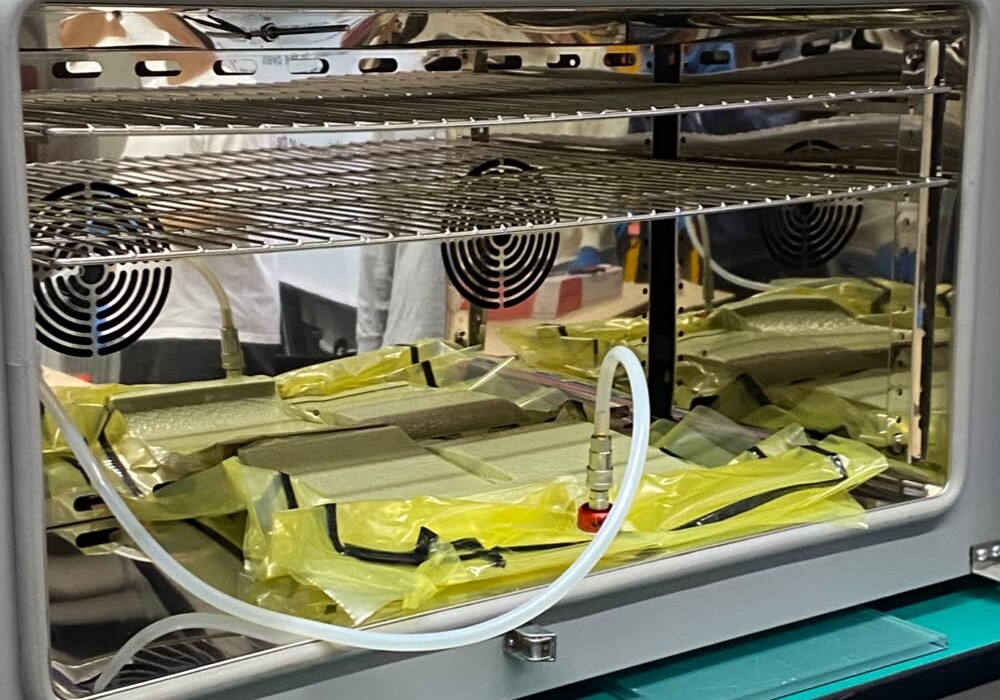
\includegraphics[width=\linewidth]{oven_bagged_moulds.jpg}\\[2pt]
        {\footnotesize (a)}
    \end{minipage}\hfill
    \begin{minipage}[b]{0.445\linewidth}
        \centering
        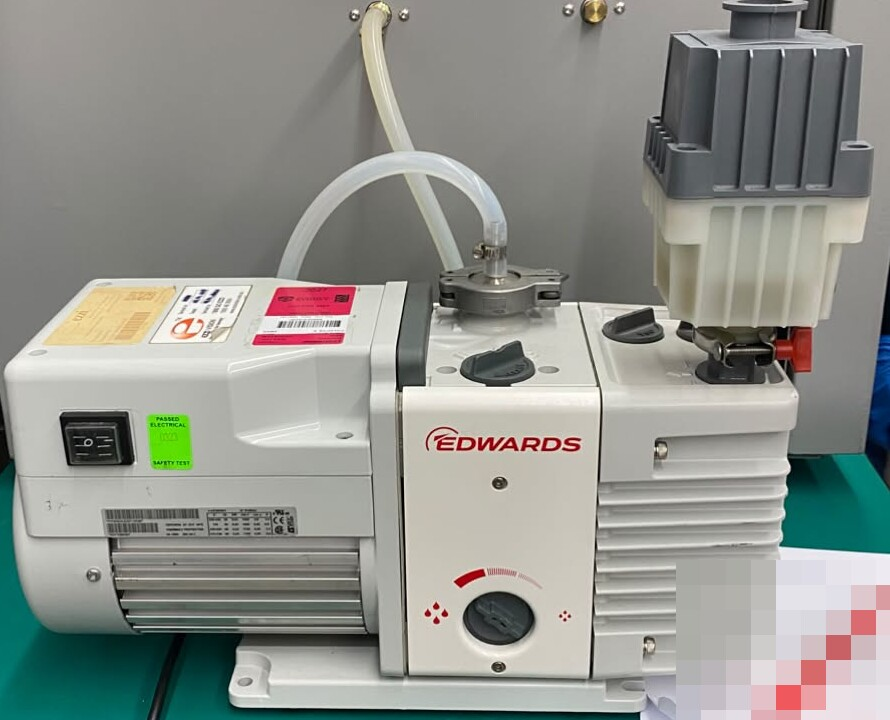
\includegraphics[width=\linewidth]{vacuum_pump.jpg}\\[2pt]
        {\footnotesize (b)}
    \end{minipage}
    \caption{Curing set-up: (a) bagged moulds in the fan-assisted oven,
    with the vacuum tubing connected to a bag's vacuum port through a
    quick-release coupling; (b) the rotary vane vacuum pump, connected
    to the oven's vacuum feed-through.}
    \label{fig:setup}
\end{figure}

\begin{addedblock}
The oven ran the four-segment programme `MECH2460'
(Figure~\ref{fig:cure}, Table~\ref{tab:cure}). It ramped from room
temperature to 60\,$^\circ$C over 35\,min ($\approx$1.1\,$^\circ$C/min,
taking room temperature as $\approx$20\,$^\circ$C), held at
60\,$^\circ$C for 60\,min, ramped to 120\,$^\circ$C over 30\,min
(2.0\,$^\circ$C/min) and held at 120\,$^\circ$C for 2\,h, a programmed
cycle of 4\,h\,5\,min. The event outputs (TS1--TS3) and the wait
function were set to zero, so each segment ran for its set time
whatever the actual chamber temperature. No cooling segment was
programmed: the parts cooled with the oven, still under vacuum, before
the bags were opened (Section~\ref{sec:procedure}, step~11).

This two-stage cycle is typical of epoxy prepregs cured under vacuum
alone. The 60\,$^\circ$C dwell lowers the resin viscosity and holds the
resin fluid, so the plies can wet out and consolidate and air trapped
between them has time to escape through the breather before the resin
gels. The faster second ramp then brings the laminate to
120\,$^\circ$C, where the 2\,h hold completes cross-linking and sets the
glass-transition temperature \citep{hexcel2013,centea2015}. The
moderate ramp rates limit thermal gradients across the aluminium
moulds, whose thermal mass makes the laminate temperature lag the oven
air temperature. Because the part temperature was not monitored with a
thermocouple, the time the laminate actually spent at 120\,$^\circ$C
was somewhat shorter than the programmed 2\,h.
\end{addedblock}

\begin{figure}[htbp]
    \addedfloat
    \centering
    \begin{minipage}[c]{0.56\linewidth}
        \centering
        \begin{tikzpicture}[font=\footnotesize, >=Stealth, black,
            x=0.0245cm, y=0.03cm]
            % axes: time 0--300 min, temperature 0--140 C
            \draw[->] (0,0) -- (315,0);
            \node[below=12pt] at (157,0) {time (min)};
            \draw[->] (0,0) -- (0,145) node[above] {temperature ($^\circ$C)};
            \foreach \t in {0,60,120,180,240,300} {
                \draw (\t,0) -- (\t,-3) node[below] {\t};}
            \foreach \T in {20,60,120} {
                \draw (0,\T) -- (-4,\T) node[left] {\T};
                \draw[gray!40] (0,\T) -- (305,\T);}
            % programmed set-point
            \draw[very thick] (0,20) -- (35,60) -- (95,60) -- (125,120) -- (245,120);
            % natural cooling (not programmed, indicative only)
            \draw[very thick, dashed, gray] (245,120) .. controls (265,85) and (285,70) .. (305,62);
            % segment labels
            \node[above, align=center, font=\scriptsize] at (17,62) {1};
            \node[above, font=\scriptsize] at (62,60) {2: dwell};
            \node[left, font=\scriptsize] at (108,93) {3};
            \node[above, font=\scriptsize] at (185,120) {4: cure hold};
            \node[right, font=\scriptsize, gray, align=left] at (268,98) {natural\\cooling};
        \end{tikzpicture}\\[2pt]
        {\footnotesize (a)}
    \end{minipage}\hfill
    \begin{minipage}[c]{0.42\linewidth}
        \centering
        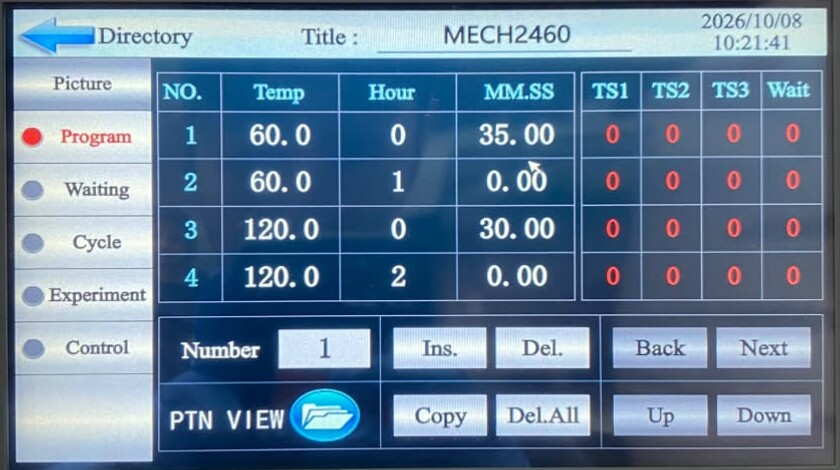
\includegraphics[width=\linewidth]{oven_program.jpg}\\[2pt]
        {\footnotesize (b)}
    \end{minipage}
    \caption{Curing temperature profile: (a) programmed oven set-point
    (solid; room temperature taken as 20\,$^\circ$C) and the
    unprogrammed natural cool-down (dashed, indicative only);
    (b) the programme on the oven controller.}
    \label{fig:cure}
\end{figure}

\begin{table}[htbp]
    \addedfloat
    \centering
    \caption{Oven programme `MECH2460' used to cure the skins.}
    \label{tab:cure}
    \small
    \renewcommand{\arraystretch}{1.1}
    \begin{tabular}{@{}cccccl@{}}
        \toprule
        \textbf{Segment} & \textbf{Target} ($^\circ$C) & \textbf{Duration}
        & \textbf{Rate} ($^\circ$C/min) & \textbf{Elapsed} & \textbf{Purpose} \\
        \midrule
        1 & 60 & 35\,min & $\approx$1.1 & 0:35 & Heat-up \\
        2 & 60 & 60\,min & 0 (dwell) & 1:35 & Resin flow, consolidation, air removal \\
        3 & 120 & 30\,min & 2.0 & 2:05 & Heat-up to cure temperature \\
        4 & 120 & 2\,h & 0 (hold) & 4:05 & Cure \\
        -- & -- & -- & -- & -- & Natural cooling under vacuum \\
        \bottomrule
    \end{tabular}
\end{table}

\begin{addedblock}
\subsection{Final Assembly and Bonding}

After cooling, the bags were cut open, the breather and peel ply were
removed and the skins were released from the moulds
(Section~\ref{sec:procedure}). Stripping the peel ply exposed the
textured bag-side surfaces, and the two skins were then placed over the
pre-shaped PU foam core and bonded with \tbc{adhesive used}
\tbc{confirm whether the bonding was done in the session or
afterwards}. The adhesive bond line adds to the section thickness, and
any mismatch between the skins and the core appears as gaps or steps
at the leading and trailing edges, so the assembled aerofoil is
expected to be slightly thicker than the nominal section formed by the
core and two 0.786\,mm skins.
\end{addedblock}
% ===================== END RESULTS (paste to here) =====================

\bibliographystyle{unsrtnat}
\bibliography{references}

\end{document}
